\addchap{Introduction}
\label{chapter:introduction}

\addchap{High Performance Computing: a story}
\label{chapter:context}

    %% TODO Historique : https://fr.wikipedia.org/wiki/Superordinateur#Historique_des_records

    \addsec{First computers}%
    \label{sec:first_computers}

        % TODO talk about the human computers, followed by the first (machine) computer created by Cray and IBM, also
        % Von Neuman, analog computers, etc.

    \addsec{Exponential growth}%
    \label{sec:exponential_growth}

        % TODO Moore's law, huge performance gains, helped to get great scientifical breakthrough
        % Not terminated yet, we "need" to go further. Side note: when will it be enough? Question of the environmental
        % impact (we make great progress in terms of efficiency, like flops/W, but the growth is even faster (so for
        % instance the total consumptions are still increasing)).

        \begin{figure}[htbp]
            \centering
            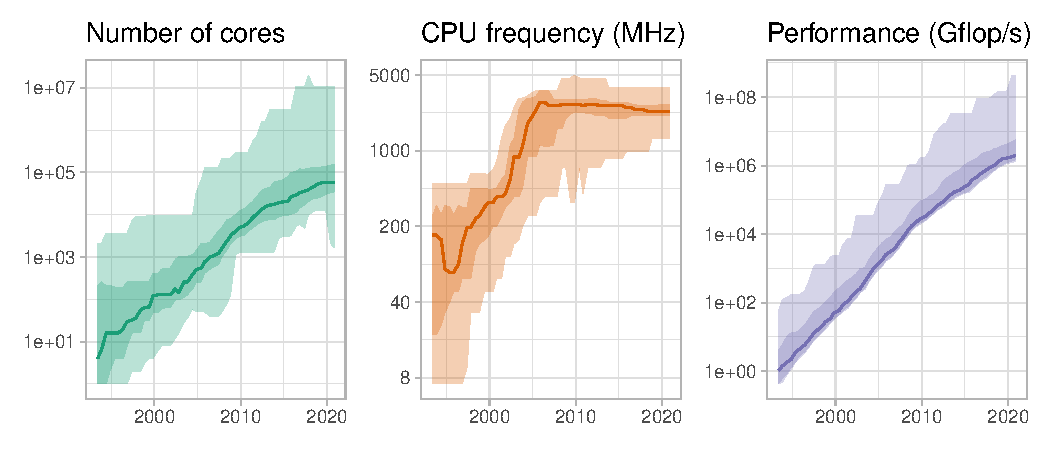
\includegraphics[width=\textwidth]{img/context/top500.pdf}
            \caption{\label{fig:context:top500}
            Both the platform performance and their total number of cores have seen an exponential increase, whereas the CPU
            frequencies have reached a plateau since 15 years}
        \end{figure}


    \addsec{Increased complexity}%
    \label{sec:increased_complexity}

        % TODO increased complexity everywhere (HW and SW), deterministic at micro-level but the macro-level is random
        % no complete understanding of the whole thing, we need experimental CS, we need models (very similarly to what
        % is done in physics or biology)
        Some horror stories\cite{Petrini_2003}\dots
